\chapter{Yauhau}

\label{chapter:Yauhau}

\yauhau{} is a compiler plugin for the Ohua compiler.
It works after the Clojure source has been parsed and transformed into the dataflow IR.
It is a pure IR to IR transformation.
Additionally a map of context information is given to the plugin.
The precise nature of this context information will be handled in section \ref{chapter:Context} and is irrelevant to for the basic \yauhau{} idea and transformation.

Fundamentally \yauhau{} performs a graph transformation on the dataflow graph it has been given in form of the IR.
The goal behind this transformation is to find rounds of IO operations which are data independent from each other and execute them as a batch job.
This is similar to the approach taken by \cite{Haxl:library:link}, a Haskell library, also with the aim of optimising IO batching.
Haxl leverages the Monad and Applicative abstractions provided by the Haskell language and base library to propagate a list of parallel executable IO actions through the program path, blocking each path as soon as an IO action is encountered.
This is a dynamic way of finding parallel IO actions, aka a runtime data structure (Data.Sequence.Seq) is populated as the program executes.
\yauhau{} takes a different approach and statically finds parallel IO actions at compile time.

\section{Runtime execution}

In \yauhau{} as well as Haxl once very remaining program path depends on data from an IO action a new round of fetches is being executed.
The list of parallel fetches is grouped into sublists on the data source they are trying to access.
Each sublist is handed to the respective datasource which has to perform the fetch.
In \yauhau{} this process is inherently parallel and each datasource performs its request at the same time in parallel.
In Haxl the programmer can choose whether to perform an asynchronous or synchronous request.
A new experimental and optional feature in \yauhau{} is to do dynamic dispatching of the finished requests.
This means once a certain datasource returns with the data computations only depending on that datasource, or an even faster one, can continue immediately.

\section{Compile time transformation}

The basic \yauhau{} transformation algorithm, as mentioned, operates entirely on a dataflow graph in form of the IR.
The transformation does not concern itself with the kinds of nodes in the graph except for one, the \texttt{fetch} node/function which is a special node provided by the \yauhau{} library.
Beyond that the algorithm only concerns itself with the structure of the graph.
This significantly simplifies the algorithm.

The goal is to find a minimal set of rounds.
A `round' is a set of \texttt{fetch} nodes with no data dependencies between the nodes.
Rounds must not overlap.
Hence the algorithm finds a minimal set of non overlapping sets of data independent \texttt{fetch nodes}.

After much consideration I decided to go for a very similar approach to Haxl by simulating running the graph and blocking code paths when a \texttt{fetch} node is encountered.
Simulating the execution of the program is done by tracking three sets of items.

\begin{description}
	\item[created] The set of created bindings tracks which pieces of data that flow between the nodes of the program have been created prior to a particular point in the program.
	\item[visited] The set of visited nodes tracks which nodes were part of a previous stage.
	\item[round] The current round consists of all \fetch{} nodes which were part of a previous stage.
	When a new fetch round is finalised it will consist of these \fetch{} nodes and the current round will be newly initialised empty.
\end{description}

Since bindings are unique in the dataflow IR we can track produced data by simply adding the respective binding to the set of created bindings.
The set of created bindings is initialised with the input parameters of our program.
From this point we traverse the graph in stages.
Each stage consists of the set of graph nodes where all inflowing data has previously been created and which was not in a previous stage.
The former condition is checked by checking, for each input binding, whether the respective binding is contained in the set of created bindings.
To ensure the latter condition a separate set of visited nodes is maintained and only nodes which are not members of this set are allowed in a new stage.
Once the stage has been computed all functions in the stage are added to the visited set.
Then all \fetch{} nodes are filtered from the stage and added to the current round.
All remaining nodes are being executed.
Simulating to executing the nodes is done by simply adding all produced binding (return bindings) of the node to the set of created bindings.
If there are no remaining nodes to execute in a stage we have reached a point where the remainder of the dataflow graph depends on IO actions, including the \fetch{} nodes.
Therefore the current round is maximal and we simulate executing all \texttt{fetch} nodes of the current round and dispatch a finalised fetch round.
Afterwards the current round set is initialised empty again.
This is done until we get an empty stage, at which point we dispatch the current round again, unless it is empty.

Adding the \fetch{} nodes to the set of visited nodes guarantees that rounds do not overlap.
Not simulating fetch execution before the round finishes guarantees that no round contains two fetches with data dependencies between them, since the dependent fetch would never have been in a stage before the round was finished since the required binding from the first fetch would not be created before the round finishes.
Finally since we only dispatch a round once no more executable nodes are found all other nodes have to be fully data dependent and this guarantees the set of rounds to me minimal minimal.
% TODO maybe actually add a proof by induction here
% Should be doable by looking at the last stage first and then working backwards to 
% previous stages.

Once the rounds have been computed an accumulated fetch is inserted for every round.
For each round all fetch nodes in the round are removed from the graph.
An accumulator is inserted with the combined inputs of all fetch nodes and the combined outputs of those nodes in the same order. See Figure \ref{figure:yauhau-transformation}.

\begin{figure}
	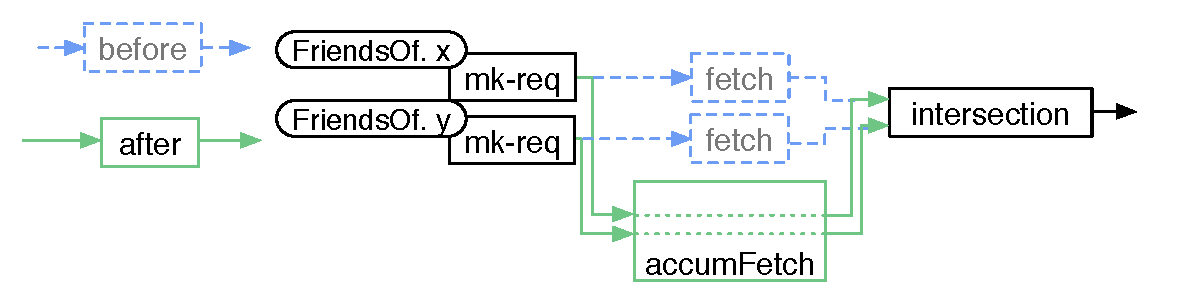
\includegraphics[width=\textwidth]{Figures/yauhau-transformation}
	\caption{base transformation}
	\label{figure:yauhau-transformation}
\end{figure}

\section{Datasources}

Datasources can be arbitrary user defined targets for IO actions such as databases, network requests or filesystem IO.
However datasources must be defined separately and only for those defined datasources the optimisation can be leveraged.

\subsection{Haxl}

Defining a datasource in Haxl means defining a set of actions on the source in form of a GADT.

\begin{minted}{Haskell}
data FacebookRequest a where
    GetFriends :: UserID -> FacebookRequest [UserID]
    GetProfile :: UserID -> FacebookRequest Profile
\end{minted}

Every time you want to make a request in the program it has to be encoded into one of those actions when passed to the IO action executing function \texttt{dataFetch}.

Additionally, for the cache, the \texttt{Hashable} typeclass needs to be implemented on this type as well as the \texttt{DataSourceName} and \texttt{StateKey} typeclass to identify the source.

The actual execution of the IO action is defined in a typeclass called \texttt{DataSource} which also has to be defined on the request type.
The \texttt{DataSource} typeclass has a method called \texttt{fetch} which does the actual work of performing the desired IO action.

\begin{minted}{Haskell}
class DataSource u request where
    fetch :: ... -> [BlockedFetch request] -> PerformFetch
\end{minted}

As its type signature indicates the \texttt{fetch} method performs the IO action on multiple requests simultaneously and this is where the batching happens.

When the framework executes the actions each datasources gets all the requests for that particular datasource. Therefore all actions which can be batched together should be defined on the same datasource (in the same GADT) and actions which cant be batched should be defined on separate datasources.

\subsection{\yauhau{}}

\yauhau{} has a more loose way of working with datasources.
IO actions in \yauhau{} are objects of the \texttt{Request} class.

\begin{minted}{Java}
public final class Request<Payload, Return>{
    private final Paylod payload;
    private final IDataSource<Payload, Return> dataSource;
    public Request(Payload payload, 
                   IDataSource<Payload, Return> dataSource) 
                  { ... }
    ...
}
\end{minted}

Each \texttt{Request} has two fields, an arbitrary Payload and a datasource.
Here the datasource, similarly to Haxl implements a Java interface \texttt{IDataSource} which provides a method for executing batched requests.

\begin{minted}{Java}
public interface IDataSource<Payload, Return> {
    Object getIdentifier();
    Iterable<Return> fetch(Iterable<Payload> requests);
}
\end{minted}

At runtime requests are sorted by the datasource they are paired with and then handed to the respective source as a single list of many requests.


















